\chapter{Design and Implementation} \label{chap:des}
This chapter covers the specific requirements for the Wireguard adaptation for GNRC, the design 
details to meet the requirements and important implementation aspects inside the Wireguard source
code for RIOT.
\section{Requirements}
  \begin{itemize}
    \item \textbf{Static memory allocation}: Dynamic memory allocation is prohibited within RIOT core 
    components to maintain a predictable runtime memory usage and real-time performance. With
    Wireguard being at layer 3 of the network stack, the protocol must use static memory
    allocation exclusively.
    \item \textbf{Security}: The GNRC implementation needs to align to the security properties that
    the original Linux implementation holds. This includes the resistance to replay attack and
    side-channel attack \cite{side}, perfect forward secrecy, low probability of handshake collision \cite{pwu},
    cryptographic soundness, and safety from concurrency bugs.
    \item \textbf{Interconnectivity with other Wireguard implementations}: The RIOT adaptation must 
    be able to communicate with other RIOT Wireguard node and obviously the Linux implementation.
    \item \textbf{Integration to RIOT network interfaces API}: Similar to the Linux implementation,
    Wireguard will be a network interface, receive IPv6 packets from the layer above, and
    handle the all the encryption and dispatching.
    \item \textbf{6LoWPAN compatibility}: The Wireguard implementation only supports IPv6 packet
    to be compatible with the 6LoWPAN layer.
  \end{itemize}
\section{Event-driven Architecture}
  Taking inspiration from BoringTun \cite{boringtun}, the Wireguard implementation handles
  packets and timers in an event-oriented manner. Three different kinds of events can occur within
  a Wireguard session:
  \begin{itemize}
    \item Transmitting data from the IP layer.
    \item Reception of a packet from any peer.
    \item The timeout event related to the Wireguard timers.
  \end{itemize}

  \begin{figure}[h]
    \centering
    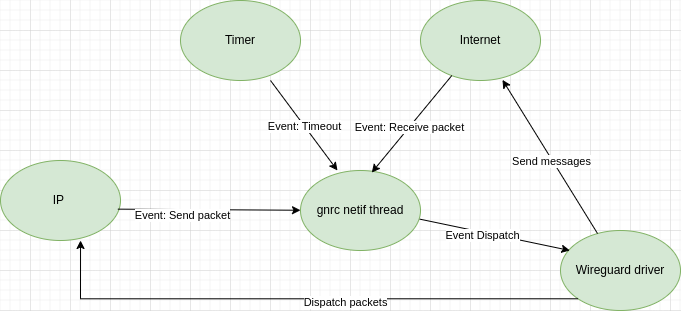
\includegraphics[width=\linewidth]{wireguard}
    \caption{GNRC Wireguard Software Architecture}
    \label{fig:wireguard}
  \end{figure}

  Figure \ref{fig:wireguard} illustrates the overview of the architecture of the GNRC Wireguard
  implementation. The Wireguard driver is the core component where it executes the Noise handshake,
  handles the functions triggered by the timeout event, encrypts, decrypts, and transmits packets to
  the IP layer or the internet outside. To make use of the existing RIOT system, the GNRC netif's
  event queue is used as the central event listener for all 3 types of events. 
  
  Whenever, a packet is received on the UDP port of Wireguard, new event to handle the reception will be pushed
  to the netif's event queue, letting Wireguard make the decision whether to respond to 
  the peer if the packet is a handshake message, dispatch the packet directly to the IP layer if 
  it is authenticated, or discard if the packet is invalid. 

  An IP layer will mostly be unaware of the inner workings of Wireguard, as it will only transmit the
  packet to the specified netif and receives the pre-processed IPv6 packet from the driver. One thing
  to note is that the Linux implementation of Wireguard will queue the packets for another thread
  to process. The GNRC also follows that design, but with a smaller packet queue to match the
  constrained environment.

  Every expiration of a timer, like the timer for retransmission of the handshake or passing the
  keepalive, the event will also be pushed on top of the event queue for the driver to handle later.
  
  The design reduces the complexity of concurrency, as every event is handled sequentially, making it impossible for 
  other threads to
  meddle with the inner cryptography state of the driver. Although it could make the netif thread
  a bottleneck of performance, the thread would not be overloaded in a normal circumstance of
  IoT environment.

\section{Network Interfaces API}
  The interface to connect to the Wireguard driver is exposed as a set of functions interacting
  with the \textbf{gnrc{\_}netif{\_}t} object. The current API is not finalized yet, and future works 
  will involve abstracting the \textbf{netif} part away, representing it as a generic Wireguard tunnel.
  Code listing \ref{lst:netifapi} shows overview of used functions to communicate with the driver.

  \begin{lstlisting}[caption = Wireguard netif API,language=C, label={lst:netifapi}]
    int gnrc_netif_wireguard_create(
      gnrc_netif_t *netif, 
      char *stack, 
      int stacksize,
      char priority, 
      char *name,
      netdev_t *dev
    );
    inline int gnrc_netif_wireguard_add_ipv6_addr(
      gnrc_netif_t *netif,
      ipv6_addr_t *addr,
      unsigned int pfx_len
    );
    void gnrc_netif_wireguard_peer_init(
      wireguard_netif_peer_t *peer
    );
    int gnrc_netif_wireguard_add_peer(
      gnrc_netif_t *netif,
      wireguard_netif_peer_t *peer,
      uint8_t *peer_idx
    );
    int gnrc_netif_wireguard_connect(
      gnrc_netif_t *netif, 
      uint8_t peer_idx
    );
    int gnrc_netif_wireguard_disconnect(
      gnrc_netif_t *netif, 
      uint8_t peer_idx
    );
  \end{lstlisting}

  The API was largely based on the API of Wireguard for the lwIP stack \cite{lwip}, with
  a bit of modification to be compatible with the RIOT API. It includes a function to 
  spawn the running \textbf{netif} thread to handle sending, receiving 
  of packet and a function to configure the IPv6 address on the network interface. 

  The \textbf{gnrc{\_}netif{\_}wireguard{\_}peer{\_}init} initializes the  memory of the struct
  \textbf{wireguard{\_}netif{\_}peer{\_}t} with default values. This netif peer represents
  the configuration of a peer object residing on the Wireguard. The corresponding
  \textbf{gnrc{\_}netif{\_}wireguard{\_}add{\_}peer} finds the free region and populates 
  the actual peer objects on the Wireguard's list. Code listing \ref{lst:netifpeer} shows
  the structure of the peer configuration. The object comprises the public key and 
  the pre-shared key for encryption decryption, the list of allowed IP addresses that the peer will
  accept, the communication endpoint, and the option to turn on/off for the persistent keepalive
  feature.

  \begin{lstlisting}[caption = netif peer configuration,language=C, label={lst:netifpeer}]
  typedef struct {
    ipv6_addr_t addr;
    unsigned int pfx_len;
  } wireguard_netif_allowed_ip_t;

  typedef struct wireguard_netif_peer {
    const char *public_key;
    const uint8_t *preshared_key;
    wireguard_netif_allowed_ip_t *allowed_ips;
    int allowed_ips_len;
    sock_udp_ep_t endpoint;
    int persistent_keepalive;
  } wireguard_netif_peer_t;
  \end{lstlisting}

  The API also supports the user to actively connect or disconnect to a peer. The connect
  functions simply register a handshake initiation transmission event, and the disconnect
  will wipe out all the symmetric keys plus any partial handshake on a peer. The intention
  for the connect function is also to reduce the number of time for queuing the transport packets,
  as the sending packets need to be queued if the session keys have not been created. 

  Later API will include shutting down all the Wireguard state gracefully, more configurations, and
  a tunnel abstraction over the netif details.

\section{Wireguard Device Driver}
  The core component of Wireguard is implemented using netdev API of RIOT. Following the specification,
  the initialization process of the driver divides into 2 steps: \textbf{wireguard{\_}setup} to prepare
  the configuration, and \textbf{wireguard{\_}init} to actually initialize the driver. 
  
  \begin{lstlisting}[caption = Wireguard driver,language=C, label={lst:wireguarddriver}]
    typedef struct wireguard_device {
      netdev_t netdev;
      wireguard_params_t *params;
      uint16_t listen_port;
      sock_udp_t udp;
      gnrc_netif_t *netif;
      event_queue_t *evq;
      struct noise_static_identity static_identity;
      struct wireguard_peers peers;
      struct cookie_checker cookie_checker;
      bool valid;
    } wireguard_t;

  \end{lstlisting}

  Listing \ref{lst:wireguarddriver} shows the data structure of Wireguard. The \textbf{netdev}
  is the parent struct to interop with the RIOT structure. The \textbf{params} field
  contains the initial configuration. The \textbf{udp} is the UDP socket connection with
  the listening port \textbf{listen{\_}port}. The peers is a thread-safe list of peers. 
  A cookie checker with the \textbf{static{\_}identity} as the static private/public keypair is
  also included. A pointer to the original network interfaces and the validity of the driver
  are required for the driver. The final important detail is the \textbf{event{\_}queue}.

  Instead of spawning a separate thread that runs on an event loop, to satisfy the memory constraint, 
  the design here is to reuse the existing event queue of \textbf{netif} to handle both reception 
  of message and timeout. However, this design has a drawback of making the sending always after the 
  event handler, due to the \textbf{netif} thread processing the awaiting events before dispatching
  the packets inside the mesage queue. Listing
  \ref{lst:netifev} illustrates this logic.

  \begin{lstlisting}[caption = Netif event handler,language=C, label={lst:netifev}]
    static void _process_events_await_msg(gnrc_netif_t *netif, msg_t *msg)
    {
        while (1) {
            /* Using messages for external IPC, and events for internal events */

            /* First drain the queues before blocking the thread */
            /* Events will be handled before messages */
            DEBUG("gnrc_netif: handling events\n");
            event_t *evp;
            /* We can not use event_loop() or event_wait() because then we would not
            * wake up when a message arrives */
            while ((evp = _gnrc_netif_fetch_event(netif))) {
                DEBUG("gnrc_netif: event %p\n", (void *)evp);
                if (evp->handler) {
                    evp->handler(evp);
                }
            }
            /* non-blocking msg check */
            int msg_waiting = msg_try_receive(msg);
            if (msg_waiting > 0) {
                return;
            }
            DEBUG("gnrc_netif: waiting for events\n");
            /* Block the thread until something interesting happens */
            thread_flags_wait_any(
              THREAD_FLAG_MSG_WAITING | THREAD_FLAG_EVENT
            );
        }
    }
  \end{lstlisting}

  Another design decision is to not implement the \textbf{send} and \textbf{recv} of the driver, but instead 
  customize an API for sending and receiving packets, where the send will handle the write-enabled 
  \textbf{pktsnip}, and the receving will take the buffer directly from the UDP socket and dispatch the packet 
  up to the IP layer if it is valid.

  The event queue also handle the triggered timer event. Each peer will maintain its own list 
  of timers, and push the callback to the event queue when the timer reach their timeout. 
  To trigger the timeout, the \textbf{event{\_}timeout{\_}t} is utilized with the \textbf{ZTIMER{\_}MSEC}
  objects. This means the time unit for the timers will be in milliseconds, allowing low-power
  sleep modes on many platforms.
\section{Memory Allocation \& Optimization}
  To reduce the memory consumption of Wireguard, 3 main points have been employed. Firstly, the default number
  of peers that a Wireguard driver can maintain is 2 peers. Hence, the user of the network interface
  API has the responsibility to manage the memory of Wireguard. As of the time of writing, the 
  feature to change the number of peers has not been actualized yet. Instead of maintaining
  a dynamic hash map like the Linux implementation to store the key pairs and the indices
  or a radix trie for the search of allowed IP address, 
  every needed state are in the peer object, a lookup is simply a linear search throughout the list of
  peers to find the required peer. An example of a look-up for allowed IP addresses is in Listing \ref{lst:allowedip}.

  \begin{lstlisting}[caption = Allowed IP address lookup,language=C, label={lst:allowedip}]
    struct wireguard_peer *
    wireguard_peer_lookup_by_allowed_ip(
      struct wireguard_peers *peers,
      const ipv6_addr_t *addr) 
    {
      struct wireguard_peer *peer = NULL;
      struct wireguard_peer *tmp;
      struct wireguard_allowed_ip *allowed;
      uint8_t best_match = 0;
      uint8_t match;
      size_t i;
      size_t j;

      mutex_lock(&peers->mtx);
      for (i = 0; i < MAX_PEERS_PER_DEVICE; ++i) {
        tmp = &peers->peers[i];
        if (!tmp->valid) {
          continue;
        }
        /* perform longest prefix match to find the dest ip */
        for (j = 0; j < MAX_SRC_IPS; ++j) {
          allowed = &tmp->allowed_source_ips[i];
          if (!allowed->valid)
            continue;
          match = ipv6_addr_match_prefix(&allowed->ip, addr);
          if (match < allowed->pfx_len)
            continue;
          /* the 0 case is when the destination allowed ip is an unspecified IPv6
          * address */
          if (match > best_match || best_match == 0) {
            peer = tmp;
            best_match = match;
          }
          /* found the exact match on the ipv6 address destination */
          if (best_match == IPV6_ADDR_BIT_LEN) {
            mutex_unlock(&peers->mtx);
            return peer;
          }
        }
      }
      mutex_unlock(&peers->mtx);
      return peer;
    }
  \end{lstlisting}

  Secondly, the driver has a global static queue for the sending packets 
  if the symmetric session keys have not been derived. The maximum number of packets that
  the queue can hold is the number of peers multiplied by two. The reason stems from the assumption
  that the period for the application to send the consecutive packets should be close to the 
  \textbf{REKEY{\_}TIMEOUT} limit, allowing a peer to retry transmitting the handshake
  while reserving the original packet in the condition of a lossy network. If a handshake 
  session can not be completed, Wireguard simply discards the queuing packets belonging
  to the peer.

  Finally, as the transport data required to be zero-padded, reallocation of the original payload
  is required. With the design of the \textbf{gnrc{\_}pktsnip{\_}t}, a packet is represented as
  a linked list of headers with the next pointer pointing to the next header or payload. To reduce
  the number of merging and reallocations, before sending the IPv6 transport payload, a special
  prepare function will compute the total required space for all encrypted payloads including
  the zero-padded trailer and the transport header, copy all header and payload into
  the reallocated data, release the hold \textbf{pktsnip}, and move the IPv6 header
  into the correct region. This is applied to the normal transport data only. For a keepalive message,
  the payload is allocated on the stack and encrypted in the same way as the transport data.
  The goal of this function is to reduce the memory fragmentation for allocation as much
  as it possibly can.
  \begin{lstlisting}[caption = The flow of transport data preparation,language=C, label={lst:prep}]
    static int wireguard_prepare_transport_snip(
      gnrc_pktsnip_t *pkt
    ) 
    {
      assert(pkt != NULL);
      size_t offset;
      size_t ipheader_offset;
      size_t plaintext_len;
      size_t trailer_len;
      size_t packet_len;
      uint8_t *buf;
      uint8_t *ip_end;
      int res = 0;

      offset = pkt->size;
      ipheader_offset = offset - 1;
      plaintext_len = gnrc_pkt_len(pkt);
      /* routnd to 16 bytes boundary */
      trailer_len =
          align_mask(plaintext_len, 16) - plaintext_len + noise_encrypted_len(0);
      packet_len = TRANSPORT_DATA_HEADER_LEN + plaintext_len + trailer_len;
      /* Re-allocate data to have enough buffer for:
      * transport_header + ipv6 packet + payload + padded 0 + auth tag*/
      res = gnrc_pktbuf_realloc_data(pkt, packet_len);
      if (res != 0) {
        DEBUG("[wireguard] send: realloc data failed");
        return res;
      }

      /* Copy data to new buffer */
      buf = ((uint8_t *)pkt->data) + TRANSPORT_DATA_HEADER_LEN;
      for (gnrc_pktsnip_t *ptr = pkt->next; ptr != NULL; ptr = ptr->next) {
        memcpy(buf + offset, ptr->data, ptr->size);
        offset += ptr->size;
      }
      /* reverse copying the ipv6 header since the transport header is shorter */
      ip_end = ((uint8_t *)pkt->data);
      /* Chapter 5.6: Mitigation Strategies for integer overflow in a reverse for
      * loop - Secure Coding in C and C++ */
      for (size_t i = ipheader_offset; i != SIZE_MAX; i--) {
        buf[i] = ip_end[i];
      }

      /* Release old pktsnips and data*/
      gnrc_pktbuf_release(pkt->next);
      pkt->next = NULL;

      return 0;
    }
  \end{lstlisting}

\section{Security Requirements \& Implementations}
  The implementation of the cryptography Noise handshake matches closely to the Linux implementation
  to ensure the correctness. All the cryptography primitives make use of the API that RIOT 
  provides. To generate the private key and cookie secretly with a low probability of predicting, SHA256
  \cite{rfc6234} pseudo-random generator is used. The ECDH function also includes an 
  additional check for zero bytes to prevent the zero bytes shared agreed key \cite{zeros}.

  Following the silent nature, an invalid packet is silently dropped, but no ICMP packet
  will be sent back to the interface. To achieve perfect forward secrecy and protect
  against various potential leaks, crypto{\_}secure{\_}wipe and crypto{\_}equals are used to
  clean up all the cryptographic state after use and safe comparison between the keys.

  Regarding the under load condition to prevent the DoS, a simple check on whether the number
  of events on the event queue is greater than 12 events is sufficient (three-quarters of 
  the limitation of the number of queued events on a thread, which is 16). The sequence space
  window algorithm \cite[appendix C]{rfc2401} is employed to protect against the transport data replay attack.

\section{Implementation Status}
  The development of Wireguard for GNRC progressed into a functional prototype with the capability
  to communicate smoothly with the Linux implementation. The prototype needs more thorough
  testing and verification and benchmarking to optimize the memory footprint and performance.
  The current implementation faces 2 important problems:
  \begin{itemize}
    \item The source code of the IP layer to allow the dispatching of IPv6 packet to the 
    Wireguard network interfaces.
    \item A direct installation of the neighbor cache entry for a socket endpoint is required to
    send the UDP packet out.
  \end{itemize}
  Finally, integrate Wireguard into \textbf{ifconfig} tool of the interactive RIOT shell is also
  an important missing feature for a smoother configuration of the interface.